\chapter{TINJAUAN PUSTAKA}

\section{Tinjauan Pustaka}
\label{sec: Tinjauan_Pustaka}
\subsection{Sistem Pelacak}
Penelitian sebelumnya telah mengembangkan berbagai sistem pelacak aset dengan berbagai macam pendekatan pada perangkat keras maupun perangkat lunak untuk berbagai aplikasi. Sebagai contoh, \cite{Ekhsan2022} merancang suatu sistem untuk melacak dompet dengan menggunakan TK-102 GPS \textit{Tracker}.

Tim peneliti dari \textit{Vidyalankar Institute of Technology} telah merancang suatu sistem yang dapat mendeteksi lokasi dari kendaraan dan juga emisi \ce{CO} yang dihasilkan. Pada sistem yang dirancang, digunakan \textit{development board} Arduino Uno yang berbasis mikrokontroler ATmega328. Ketika kandungan gas \ce{CO} sudah melebihi ambang batas, sistem akan memutus pengiriman bahan bakar dan kemudian mengirimkan data koordinat dari modul GPS ke \textit{server} Apache yang telah dirancang \cite{Asha2022}.

Sebuah sistem \textit{speedometer} telah dirancang oleh \cite{Najmurrokhman2021}. Sistem tersebut menggunakan modul GPS untuk menghitung kecepatan dan koordinat lokasi kendaraan. Data kecepatan kendaraan didapat dari menghitung waktu yang dibutuhkan oleh kendaraan untuk berpindah dari satu titik ke titik lainnya. Data yang didapat dikirimkan dengan API Adafruit IO menggunakan modul SIM808.

Penelitian yang dilakukan oleh \cite{Mukhtar2015} dari \textit{University of London} menggunakan mikrokontroler AT89S52 dari keluarga 8051. Digunakan modul GPS M-89 yang diatur untuk menerima isyarat transmisi satelit pada frekuensi 1575.42 MHz. Data yang diterima akan ditampilkan pada layar LCD dan dikirimkan dengan modul GSM. Kemudian, data yang telah diterima akan ditampilkan pada situs web.

\section{Dasar Teori}
\subsection{Pita L}

\subsection{Teknologi GNSS}
\textit{Global Navigation Satellite System} (GNSS) adalah istilah yang digunakan untuk suatu sistem navigasi radio yang menggunakan konstelasi satelit. Salah satu contoh GNSS adalah \textit{Global Positioning System} (GPS) milik Amerika Serikat. Selain GPS terdapat lima sistem GNSS lainnya yaitu, Galileo (Uni Eropa), BeiDou (Republik Rakyat Tiongkok), GLONASS (Federasi Rusia), IRNSS (India), dan QZSS (Jepang) \cite{NationalCoordinationOfficeforSpace-BasedPositioning2021}. Sistem GNSS bekerja dengan cara mengobservasi jarak antara penerima dengan satelit \cite{TheEuropeanGlobalNavigationSatelliteSystemsAgency2021}. Satelit GNSS akan terus memancarkan isyarat radio pada pita frekuensi L.

\begin{figure}[ht]
	\centering
	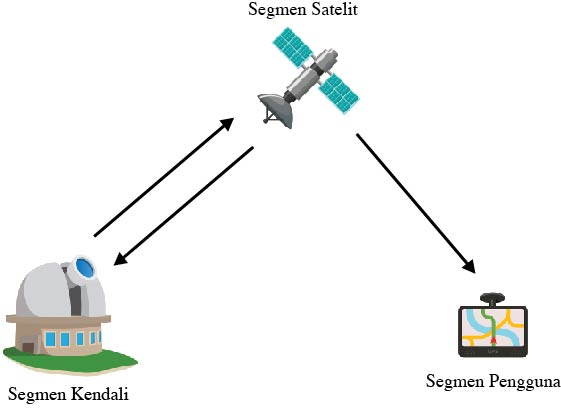
\includegraphics[width=8cm]{contents/chapter-2/gnss_segment.jpg}
	\caption{\textit{Segmen GNSS}}
	\label{Fig: gnss_segment}
\end{figure}

Setiap GNSS terdiri dari tiga buah segmen, yaitu segmen satelit sebagai pemancar isyarat, segmen kendali untuk injeksi data dan memantau performa satelit, dan segmen pengguna. Hubungan dari ketiga segmen GNSS ditunjukan oleh Gambar \ref{Fig: gnss_segment}. 

\subsubsection{Trilaterasi}
\begin{figure}[ht]
	\centering
	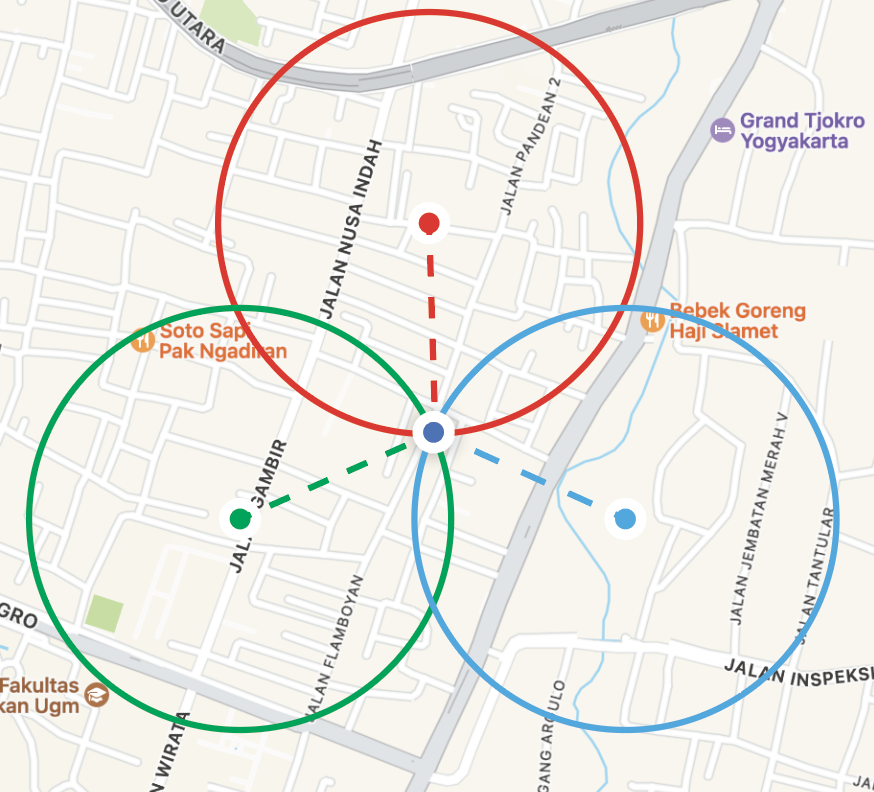
\includegraphics[width=8cm]{contents/chapter-2/trilaterasi.png}
	\caption{Trilaterasi}
	\label{Fig: Trilaterasi}
\end{figure}
Trilaterasi adalah proses menentukan posisi berdasarkan jarak dengan menggunakan setidaknya tiga buah satelit \cite{AmericanSocietyofCivilEngineers1994}. Ilustrasi dari trilaterasi sederhana dengan tiga buah satelit dapat dilihat pada Gambar \ref{Fig: Trilaterasi}. Misalkan titik merah, hijau, dan biru muda adalah letak dari tiga satelit dan lingkaran di sekitarnya adalah jangkauan dari masing-masing satelit pada bidang dua dimensi. Terlihat bahwa perkiraan lokasi pada objek adalah irisan dari ketiga lingkaran tersebut (titik berwarna biru tua). Perhitungan trilaterasi akan dibahas pada bagian selanjutnya \cite{Seo2012}.

Posisi objek pada bidang dua dimensi dengan Trilaterasi 2D dapat didapatkan dengan menyelesaikan persamaan berikut
\begin{equation}
	\left(x-x_1\right)^2 + \left(y-y_1\right)^2=d_1^2
	\label{eq:2-1}
\end{equation}
\begin{equation}
	\left(x-x_2\right)^2 + \left(y-y_2\right)^2=d_2^2
	\label{eq:2-2}
\end{equation}
\begin{equation}
	\left(x-x_3\right)^2 + \left(y-y_3\right)^2=d_3^2
	\label{eq:2-3}
\end{equation}
Persamaan \ref{eq:2-1}, \ref{eq:2-2}, dan \ref{eq:2-3} dapat diubah menjadi persamaan linear dengan melakukan substitusi, sehingga didapat
$$2\left(x_2-x_1\right)x +2 \left(y_2-y_1\right)y=\alpha$$
$$2\left(x_3-x_1\right)x+ 2\left(y_3-y_1\right)y=\beta$$
dengan
$$\alpha=\left(d_1^2-d_2^2\right)-\left(x_1^2-x_2^2\right)-\left(y_1^2-y_2^2\right)$$
$$\beta=\left(d_1^2-d_3^2\right)-\left(x_1^2-x_3^2\right)-\left(y_1^2-y_3^2\right).$$
Posisi $\left(x,y\right)$ didapat dengan menyelesaikan persamaan matriks berikut
$$x=f\left(d_1,d_2,d_3\right)=\frac{
	\begin{vmatrix}
		\alpha & 2Y_1^2 \\
		\beta & 2Y_1^3 \\
\end{vmatrix}}
{
	\begin{vmatrix}
		2X_1^2 & 2Y_1^2 \\
		2X_1^3 & 2Y_1^3 \\
	\end{vmatrix}
}$$
$$y=g\left(d_1,d_2,d_3\right)=\frac{
	\begin{vmatrix}
		2X_1^2 & \alpha \\
		2X_1^3 & \beta \\
\end{vmatrix}}
{
	\begin{vmatrix}
		2X_1^2 & 2Y_1^2 \\
		2X_1^3 & 2Y_1^3 \\
	\end{vmatrix}
}$$
dengan $X_i^j$ dan $Y_i^j$ adalah $\left(x_i-x_j\right)$ dan $\left(y_i-y_j\right)$.

Trilaterasi 3D dapat dilakukan dengan memodifikasi persamaan \ref{eq:2-1}, \ref{eq:2-2}, dan \ref{eq:2-3} dan mengulangi langkah-langkah pada Trilaterasi 2D. Untuk menentukan posisi $\left(x,y,z\right)$ objek pada bidang tiga dimensi dapat dilakukan dengan menyelesaikan persamaan matriks berikut
$$
\hat{x}=\hat{f}\left(d_1,d_2,d_3\right)=\frac{
	\begin{vmatrix}
		\alpha & 2Y_1^2 & 2Z_1^2\\
		\beta & 2Y_1^3 & 2Z_1^3\\
		\gamma & 2Y_1^4 & 2Z_1^4
\end{vmatrix}}
{
	\begin{vmatrix}
		2X_1^2 & 2Y_1^2 & 2Z_1^2\\
		2X_1^2 & 2Y_1^3 & 2Z_1^3\\
		2X_1^2 & 2Y_1^4 & 2Z_1^4
	\end{vmatrix}
}
$$
$$
\hat{y}=\hat{g}\left(d_1,d_2,d_3\right)=\frac{
	\begin{vmatrix}
		2X_1^2 & \alpha & Z_1^2\\
		2X_1^3 & \beta & 2Z_1^3\\
		2X_1^4 & \gamma & 2Z_1^4
	\end{vmatrix}
}
{
	\begin{vmatrix}
		2X_1^2 & 2Y_1^2 & 2Z_1^2\\
		2X_1^2 & 2Y_1^3 & 2Z_1^3\\
		2X_1^2 & 2Y_1^4 & 2_1^4
	\end{vmatrix}
}
$$
$$\hat{z}=\hat{h}\left(d_1,d_2,d_3\right)=\frac{
	\begin{vmatrix}
		2X_1^2 & 2Y_1^2 & \alpha\\
		2X_1^3 & 2Y_1^3  & \beta\\
		2X_1^4 & 2Y_1^4 & \gamma
\end{vmatrix}}
{
	\begin{vmatrix}
		2X_1^2 & 2Y_1^2 & 2Z_1^2\\
		2X_1^2 & 2Y_1^3 & 2Z_1^3\\
		2X_1^2 & 2Y_1^4 & 2+_1^4
	\end{vmatrix}
}
$$
\subsubsection{Penerima GNSS}
Penerima GNSS adalah bagian dari segmen pengguna. Isyarat yang dikirimkan oleh satelit berisi efemeris, almanak, dan komponen lainnya seperti tanggal dan status satelit.

\begin{figure}[ht]
	\centering
	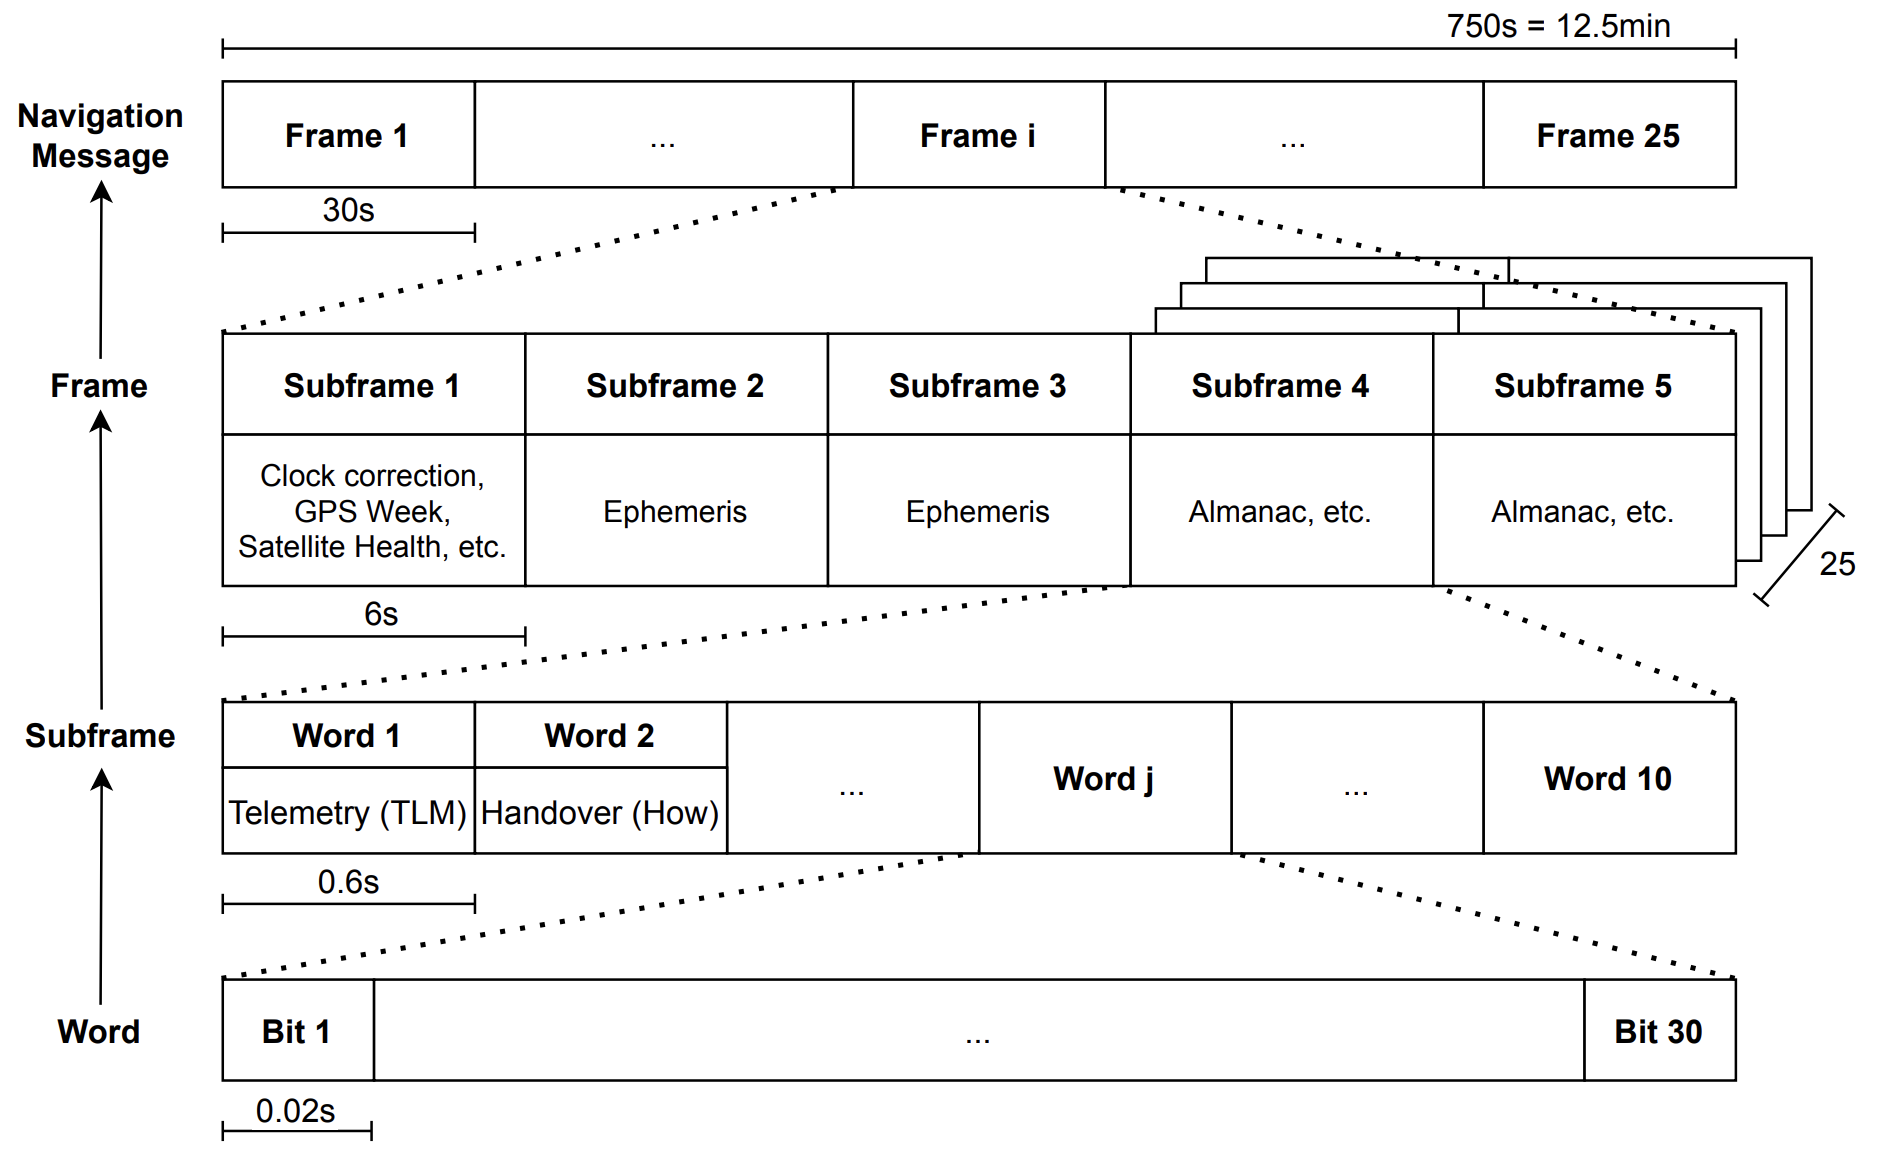
\includegraphics[width=13cm]{contents/chapter-2/gnss_msg_structure.png}
	\caption{Struktur pesan C/A NAV GNSS}
	\label{Fig: gnss_message_structure}
\end{figure}

Gambar \ref{Fig: gnss_message_structure} menunjukan lima \textit{sub-frame} pada pesan yang diterima. Efemeris berisi informasi keadaan satelit dan posisinya pada orbit, sedangkan almanak berisi informasi yang lebih umum mengenai posisi pada orbit \cite{Lenhart2022}. Dibutuhkan waktu 12.5 menit untuk mengunduh almanak dan 18 detik untuk mengunduh efemeris. Ketika modul GNSS diaktifkan untuk pertama kali maka ia akan mengunduh data tersebut dan melakukan fiksasi terhadap tiga (2D) atau empat (3D) buah satelit. Proses tersebut dikenal sebagai \textit{cold start}.

\subsection{STM32 Nucleo-WL55JC1}
STM32 Nucleo-WL55JC1 adalah \textit{development board} berbasis mikrokontroler STM32WL55 yang  dikembangkan oleh ST Microelectronics. Mikrokontroler yang digunakan adalah STM32WL55  \textit{dual-core }Arm Cortex-M4/M0+ dengan \textit{clock speed} 48 MHz \cite{STMicroelectronics2022a}.

\begin{figure}[ht]
	\centering
	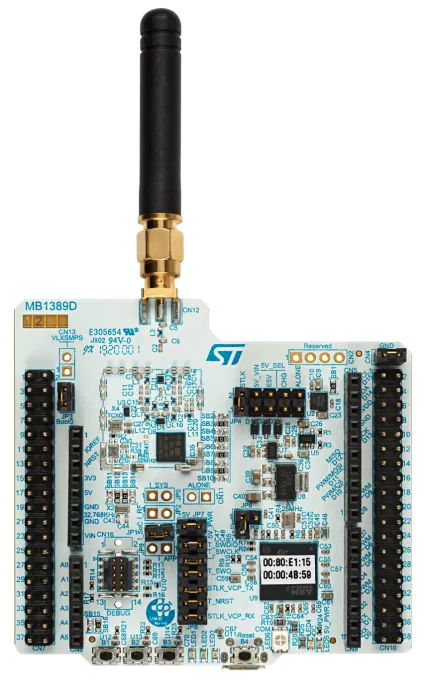
\includegraphics[width=5cm]{contents/chapter-2/stm32-wl55jc1.jpg}
	\caption{\textit{Development board} STM32 Nucleo-WL55JC1}
	\label{Fig: STM32 Nucleo-WL55JC1}
\end{figure}

Perangkat ini sudah terintegrasi dengan STLINK-V3E, sehingga tidak dibutuhkan perangkat tambahan untuk memrogram dan melakukan \textit{debugging} pada perangkat \cite{STMicroelectronics2022}. Selain itu, perangkat ini juga mendukung penggunaan \textit{expansion board} Arduino dan ST morpho. \textit{Development board} STM32 Nucleo-WL55JC1 ditunjukan oleh Gambar \ref{Fig: STM32 Nucleo-WL55JC1}.

Mikrokontroler STM32WL55 memiliki \textit{clock speed} 48 MHz jika dibandingkan dengan Arduino Mega yang hanya 16 MHz. Selain itu, STM32WL55 memiliki SRAM dengan kapasitas 64 KB atau delapan kali lipat dari yang dimiliki oleh Arduino Mega \cite{STMicroelectronics2022b}.

Karena performa tinggi dengan konsumsi daya rendah, maka digunakan mikrokontroler STM32WL55. Selain itu, STM32 juga memiliki komunitas yang tidak kalah luas dengan komunitas Arduino dan ESP-32.

\subsection{Teseo-LIV3FL}
Teseo-LIV3FL adalah modul GNSS yang diproduksi oleh STMicroelectronics. Modul ini mendukung berbagai konstelasi (GPS, GLONASS, Galileo, QZSS, dan BeiDou) \cite{STMicroelectronics2022}. 
Ukuran dari modul ini adalah 9.7 x 10.1 mm dengan osilator RTC yang dapat mengurangi TTFF. Modul Teseo-LIV3FL mendukung komunikasi secara UART dan I2C seperti yang ditunjukan pada Gambar \ref{Fig: teseo_pinout}.
\begin{figure}[ht]
	\centering
	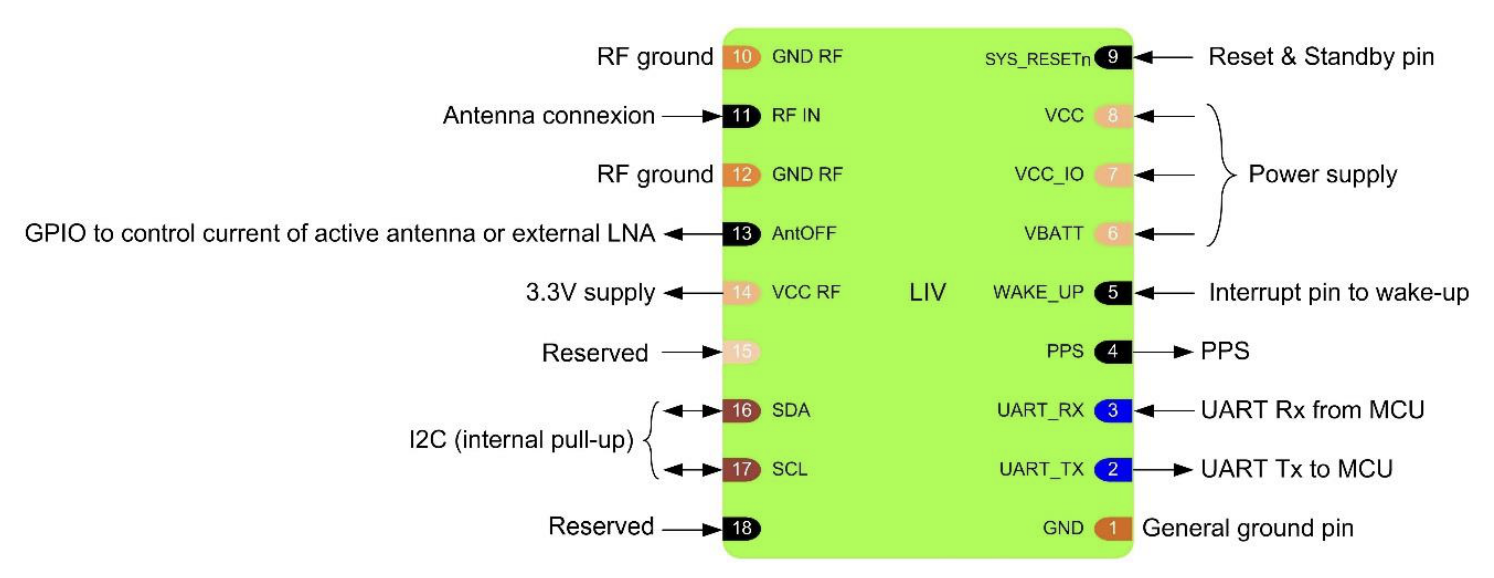
\includegraphics[width=13cm]{contents/chapter-2/teseo_pinout.png}
	\caption{\textit{Pinout} Teseo-LIV3FL \cite{STMicroelectronics2022a}}
	\label{Fig: teseo_pinout}
\end{figure}

Kelebihan dari modul Teseo-LIV3FL adalah membutuhkan daya rendah untuk mengoperasikannya (8$\mu$A mode \textit{standby} dan 45mA mode akuisisi). Nilai tersebut lebih kecil jika dibandingkan dengan modul GNSS lainnya (u- blox Neo-6M) yang membutuhkan 11 s.d. 47mA \cite{U-blox2011}. Selain itu, modul Teseo-LIV3FL juga terintegerasi dengan aplikasi Teseo-Suite yang memudahkan pengguna untuk mengunggah pengaturan modul GNSS.